% 学習結果説明（手順3e：キャビティ厚み H を入力にすることの検討。用語集と図の見方）
% results フォルダで「lualatex 学習結果説明_手順3e.tex」を2回実行すると PDF を作り直せる（TeX Live の LuaLaTeX を使用）。
% 図は results/step3e/ の PNG を相対パスで読み込む。
\documentclass[paper=a4paper,fontsize=10.5pt,line_length=44zw,number_of_lines=38]{jlreq}
\usepackage[haranoaji]{luatexja-preset}
\usepackage{amsmath}
\usepackage{graphicx}
\usepackage{booktabs}
\usepackage{tabularx}
\usepackage{enumitem}
\usepackage{float}
\usepackage{xcolor}
\usepackage[hidelinks,bookmarksnumbered]{hyperref}
\graphicspath{{step3e/}}

\newcommand{\file}[1]{\texttt{\detokenize{#1}}}
\newcommand{\gd}{\dot{\gamma}}
\newcommand{\Tff}{T_{\mathrm{ff}}}
\newcommand{\Tset}{T_{\mathrm{set}}}
\newcommand{\PI}{P3\_1}
\newcommand{\PII}{P3\_2}
\newenvironment{termlist}{\begin{itemize}[label=・,leftmargin=1\zw,labelwidth=1\zw,labelsep=0pt,itemsep=0.4ex,topsep=0.6ex,parsep=0pt]}{\end{itemize}}
\newcommand{\term}[1]{\item \textbf{#1}：}
\newenvironment{points}{\begin{itemize}[label=$\triangleright$,leftmargin=1.5\zw,itemsep=0.3ex,topsep=0.5ex,parsep=0pt]}{\end{itemize}}
\newcommand{\pt}[1]{\item \textbf{#1}：}
\renewcommand{\arraystretch}{1.25}

\title{樹脂粘度モデル開発　手順3eの学習結果の説明\\[0.6ex]{\large キャビティ厚み $H$ を入力にすることの検討（リークか、Cross-WLF と同じ変数で足りるか）：用語集とグラフの見方（機械学習・統計を初めて学ぶ人向け）}}
\author{}
\date{2026年10月14日}

\begin{document}
\maketitle
{\small\tableofcontents}

% =====================================================================
\section{この文書について}

この文書は、\file{results/step3e/} にある手順3eの結果（図と表）を、機械学習や統計を初めて学ぶ人でも読めるように説明したものです。手順3e は、ユーザーの問い（2026 年 10 月 14 日）を調べた手順です。

\begin{quote}
キャビティ厚み $H$ は、目的変数（樹脂粘度）を算出するときの流量の計算に使われる値なので、入力に使うとリークではないか。Cross-WLF モデルの入力には厚みがないので、厚みを入力にする学習方法には疑問がある。
\end{quote}

\begin{points}
\pt{対象の結果}\file{results/step3e/}：図 4 枚、CSV 5 個。図は、すべて \file{results/step3e/highres/} にも 600 dpi で保存されます（ほかに、せん断速度 ― 粘度のグラフ 42 枚）。
\pt{読み方}2章で何を調べたかをつかみ、分からない言葉は3章の用語集で調べてください。4章で図の見方、5章で表の見方、6章で結論と、これからの選択肢を説明します。\textbf{結論だけを知りたいときは、6章から読んでください}。
\pt{元のノート}\file{01_機械学習コードフォルダ} の \file{手順3e_厚みHの扱い.ipynb} です。実行は約 20 分です。
\pt{記号表}記号・モデル名・列名の一覧は、\file{学習結果説明_記号表.pdf} にあります。
\pt{作り直し方}\file{results} フォルダで \texttt{lualatex 学習結果説明\_手順3e.tex} を2回実行すると、この PDF を作り直せます。
\end{points}

% =====================================================================
\section{何を調べたか（概要）}

\subsection{リークとは}
\textbf{リーク}（目的変数の漏れ）は、入力の中に、答え（目的変数）を作るのに使った情報が紛れ込み、モデルが「物の性質」ではなく「答えの計算のしかた」を覚えてしまうことです。次のどちらかに当たると、リークと考えます。
\begin{enumerate}[itemsep=0.3ex,topsep=0.5ex]
\item \textbf{入力から、答えが計算できてしまう}：入力の値を算出式に入れると、答えがほぼそのまま出てくる。
\item \textbf{予測するときに、その入力が分からない}：その入力は、答えと同時に、流れの結果として測られる値で、成形条件から予測するときには、まだ分からない。
\end{enumerate}
手順2・3a で見つけた圧力（\PI）は、両方に当たりました。

\subsection{算出式}
\begin{table}[H]
\caption{見かけの粘度の算出式（スリット近似。$L$ = 17.5 mm はセンサ間距離、$W$ は幅、$\Delta t$ は 2 点への到達の時間差、$\Delta P$ は圧力差）}\label{tab:eq}
\begin{tabularx}{\linewidth}{@{}l>{\raggedright\arraybackslash}p{13\zw}X@{}}
\toprule
量 & 式 & $\ln$ をとると \\
\midrule
流量 & $Q = W H L/\Delta t$ & \\
見かけのせん断速度 & $\gd = 6Q/(W H^2) = 6L/(H\,\Delta t)$ & $\ln\gd = -\ln H - \ln\Delta t$ ＋ 定数 \\
見かけの壁面せん断応力 & $\tau = \Delta P\,H/(2L)$ & $\ln\tau = \ln\Delta P + \ln H$ ＋ 定数 \\
見かけの粘度 & $\eta = \tau/\gd = \Delta P\,H^2\,\Delta t/(12L^2)$ & $\ln\eta = \ln\Delta P + \ln H - \ln\gd$ ＋ 定数 \\
\bottomrule
\end{tabularx}
\end{table}
$\ln\eta$ は、$\Delta P$（流れの結果として測る値）、$H$（金型の寸法。事前に決まる）、$\gd$（測った $\Delta t$ と $H$ から計算）の 3 つで決まります。$\Delta P$ を入力に入れると、$\ln\eta$ を計算できてしまいます（リーク）。$H$ と $\gd$ だけでは、$\Delta P$ が分からないので、計算できないはずです。これを、データで確かめました（3 節の表\ref{tab:form}）。

\subsection{理想的なスリット流れでは、見かけの流動曲線は厚みによらず重なる}
等温で、壁に固化層ができず、壁面ですべりもない、理想的なスリット流れでは、見かけの粘度と見かけのせん断速度の関係（見かけの流動曲線）は、\textbf{厚みによらず 1 本に重なります}。見かけの値と真の値の換算（ラビノビッチの補正）は、流動曲線の傾きだけで決まり、厚みに関係しないためです（スリットやキャピラリーの寸法を変えて、流動曲線が重なるかで、壁面すべりなどを調べる方法〔Mooney の方法〕の前提です）。

したがって、\textbf{厚みで流動曲線がずれるなら、そのずれは、計算の都合（$H$ を式に使ったこと）ではなく、流れの中で実際に起きている現象}（冷却、壁にできる固化層、せん断発熱など）によるものです。

\subsection{比べたモデル}
\begin{table}[H]
\caption{比べたモデル（GPR。ARD Matern 5/2 ＋ 線形カーネル ＋ ノイズ。$\gd$ は条件平均。データは手順3d の 2 つの版）}\label{tab:models}
\begin{tabularx}{\linewidth}{@{}l>{\raggedright\arraybackslash}p{11\zw}X@{}}
\toprule
記号 & 入力 & 位置づけ \\
\midrule
R3 & $\gd$，$\ln H$，$\Tset$ & 基本のモデル（手順3b） \\
RFo & $\gd$，$\ln\mathrm{Fo}$，$\Tset$ & R3 の $H$ をフーリエ数に替える。$\ln\mathrm{Fo} = -(\ln\gd + 3\ln H)$ ＋ 定数 なので、$H$ と同じ情報。構造 A・B の入力 \\
W0 & $\gd$，$\Tset$ & \textbf{Cross-WLF と同じ変数}（温度は設定温度）。$H$ を外す \\
W1 & $\gd$，$\ln\Tff$ & \textbf{Cross-WLF と同じ変数}（温度は、流れの中の樹脂温度。Cross-WLF の $T$ に近い）。$H$ を外す \\
W1T & $\gd$，$\ln\Tff$，$\Tset$ & 参考。$H$ を外し、2 つの温度 \\
\bottomrule
\end{tabularx}
\end{table}
評価は、5data 版の S\_V（外挿）・S\_T（210 ℃）と、Alldata 版の CV（条件単位の 10 分割）です。

% =====================================================================
\section{用語集}
\begin{termlist}
\term{リーク}2.1 節。入力から答えが計算できてしまう、または、予測のときに分からない値を入力に使うこと。
\term{見かけの流動曲線}見かけのせん断速度と、見かけの粘度の関係を、両対数で描いた曲線。
\term{理想的なスリット流れ}等温で、固化層も、壁面すべりもない流れ。見かけの流動曲線が、厚みによらず重なる。
\term{固化層}金型の壁で冷やされて固まった樹脂の層。流れられる隙間が、実際の厚みより狭くなる。薄い厚みほど、隙間に占める割合が大きい。
\term{フーリエ数（Fo）}冷却の度合いを表す数。$\mathrm{Fo} = \alpha\,\Delta t/H^2$（$\alpha$ は熱拡散率）。流れる時間が長く、厚みが薄いほど大きい（よく冷える）。
\term{Cross-WLF モデル}射出成形の流動解析で使われる、樹脂の粘度の式。入力は、せん断速度 $\gd$、温度 $T$、圧力 $P$。厚みは入力にない。流動解析のソフトでは、厚みの効果（冷却・固化層）は、解析の側（厚み方向の温度や固化層を計算する）で扱う。
\term{材料の式と、見かけの値のモデル}材料の式（Cross-WLF など）は、その場の $\gd$・$T$・$P$ で決まる、材料そのものの性質。この研究の目的変数は、冷却・固化・発熱の効果を含んだ「見かけの粘度」（CLAUDE.md §2）で、材料の性質と、流れ方（厚み・時間）の両方を含む。
\term{純粋誤差（ノイズの床）}同じ条件のショット間のばらつき（$\ln\eta$ の標準偏差。約 0.04）。成形条件だけを入力にしたモデルは、これより小さい誤差にはなれない。リークがあると、これより小さくなる。
\term{長さスケール}ARD の、入力ごとの値。小さいほど、その入力の小さな変化で、出力が大きく変わる。下限（0.01）に張り付くと、その入力の値を「目印」にして、条件を一つずつ覚えている状態。
\term{RMSE・被覆率}手順3a・3b の用語集と同じ（予測の平均的な誤差、95\% 予測区間に実測が入った割合）。
\end{termlist}

% =====================================================================
\section{図の見方}

% ---------------------------------------------------------------------
\subsection{図1：厚みごとの見かけの流動曲線（\file{fig1\_flow\_curves\_by\_thickness.png}）}
\begin{figure}[H]
\centering
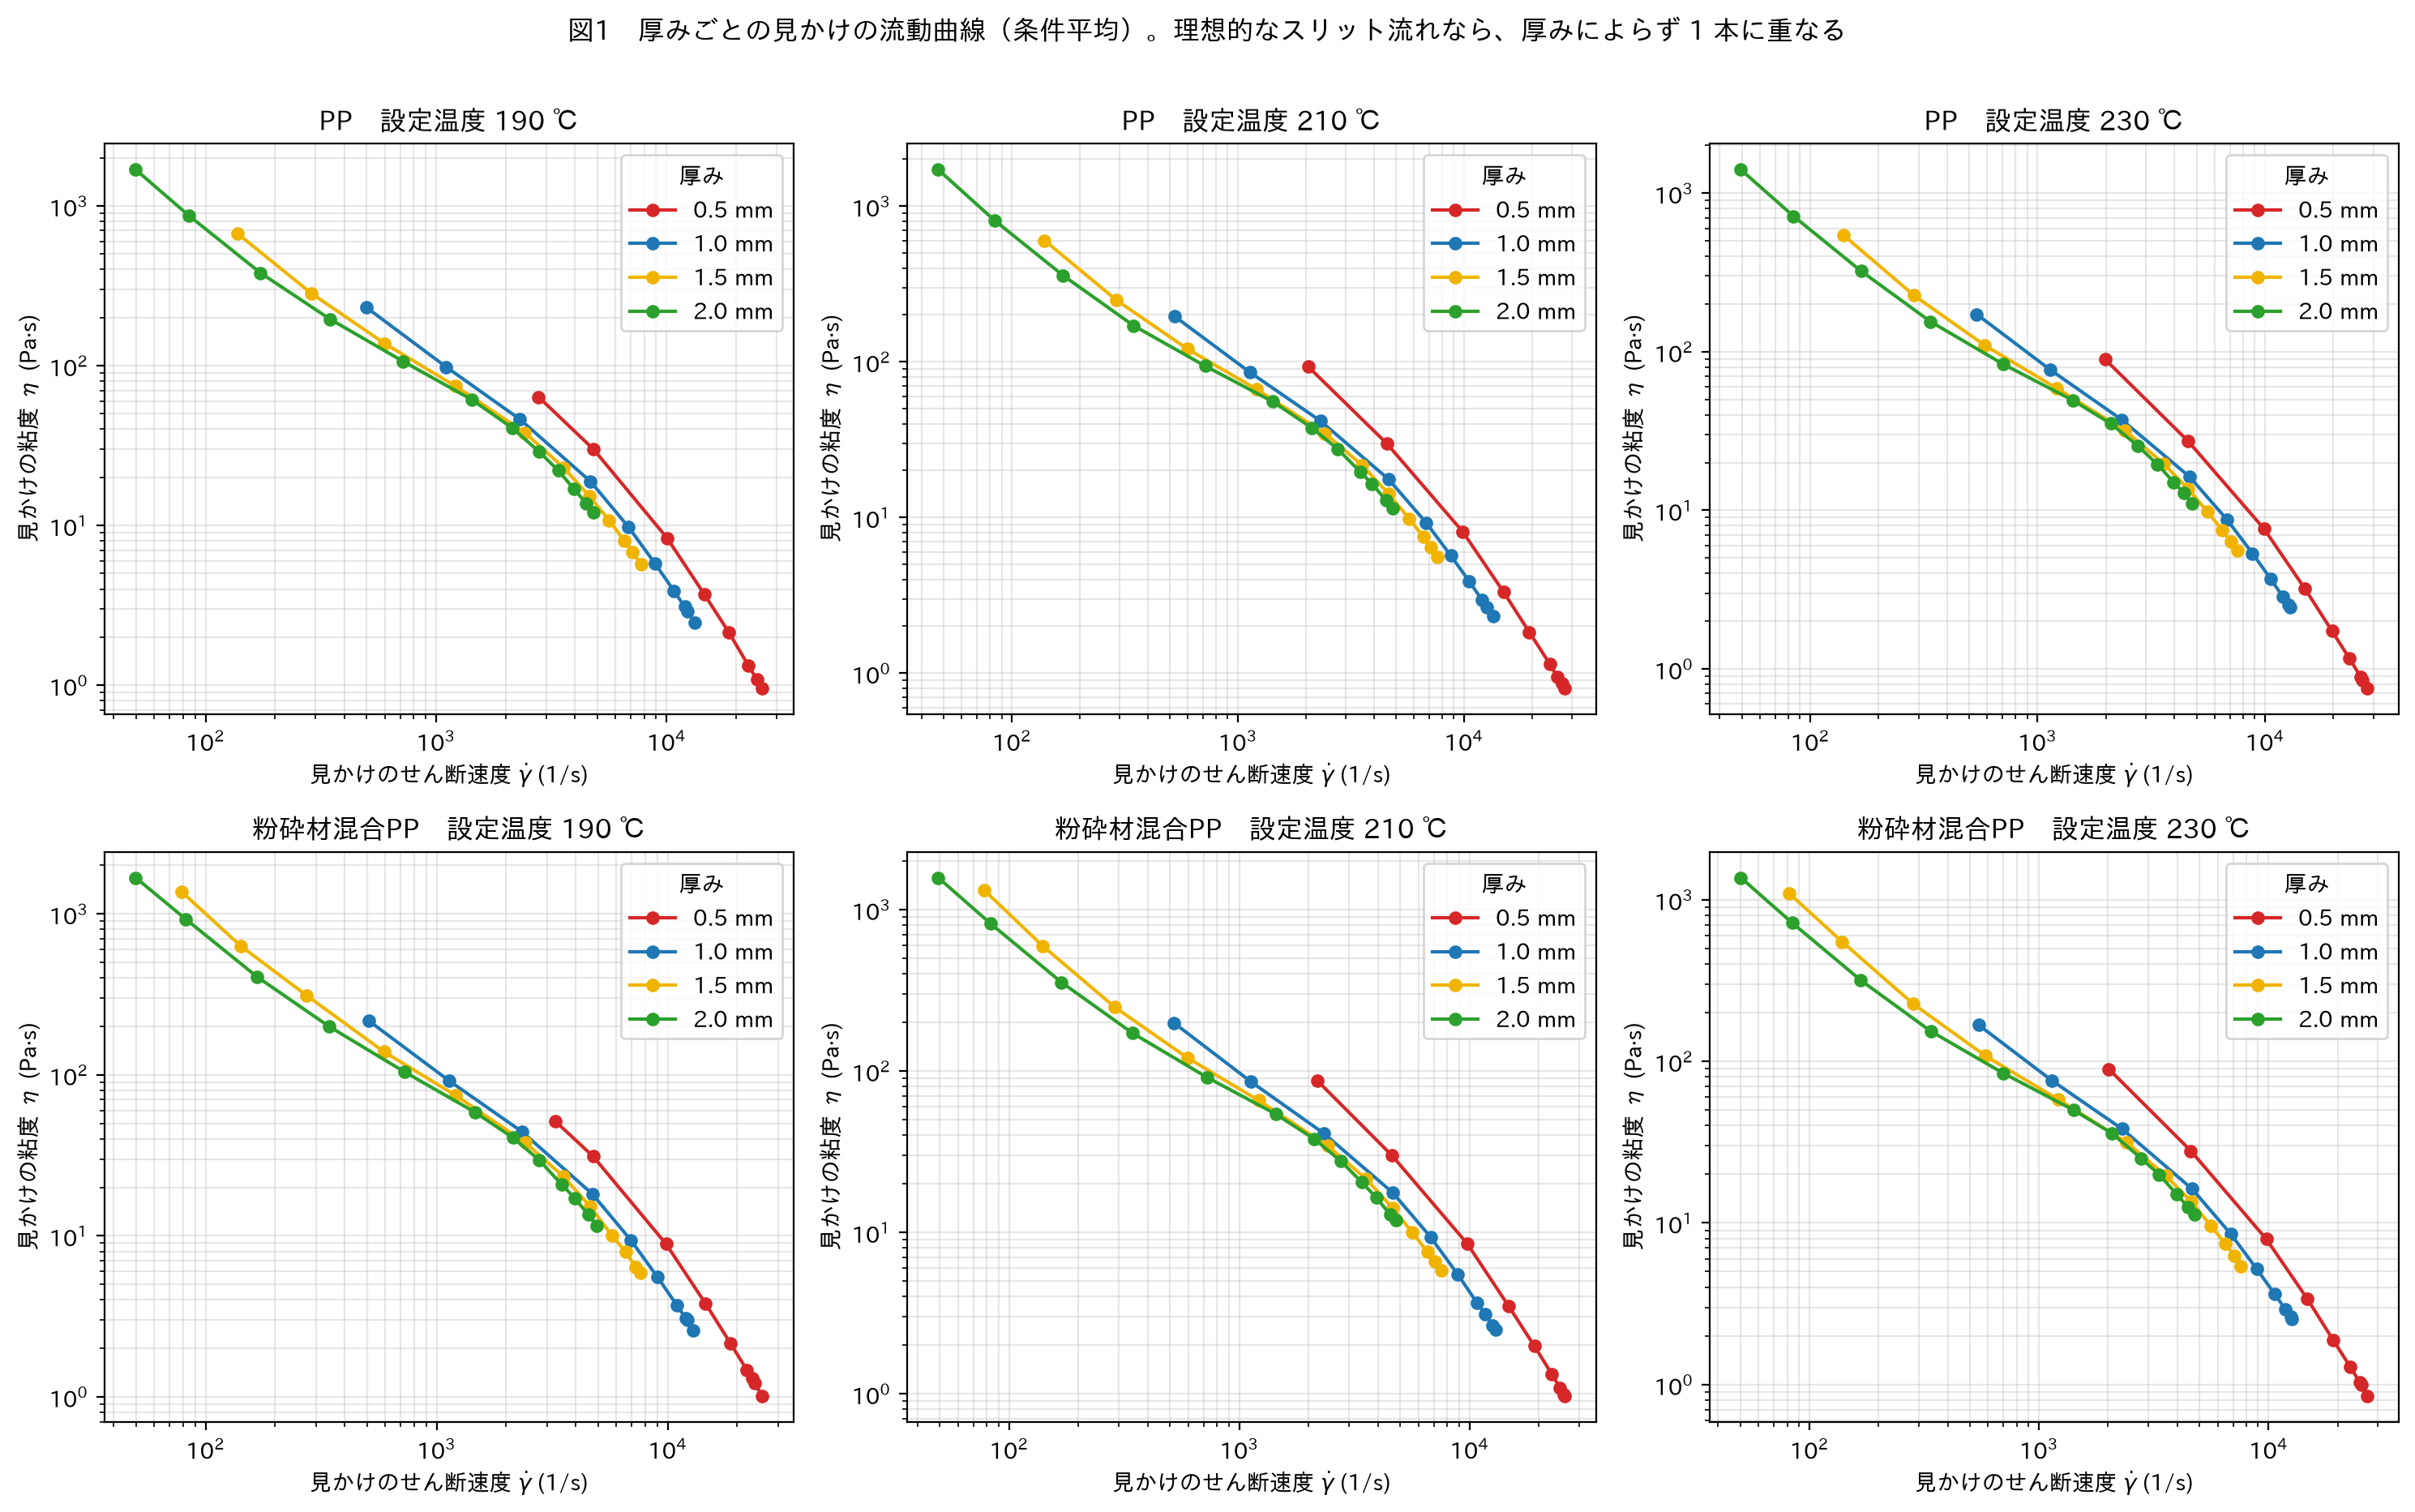
\includegraphics[width=\linewidth]{fig1_flow_curves_by_thickness.png}
\caption{厚みごとの見かけの流動曲線（条件平均。上が PP、下が粉砕材混合 PP。列が設定温度）}
\end{figure}
\begin{points}
\pt{何を示す図か}同じ設定温度で、厚みごとに、見かけの流動曲線を並べた図です。
\pt{軸と記号}横軸は見かけのせん断速度、縦軸は見かけの粘度（両対数）。色が厚み（赤 0.5 mm、青 1.0 mm、黄 1.5 mm、緑 2.0 mm）。点は条件平均。
\pt{見るポイント}理想的なスリット流れなら、4 本の曲線は 1 本に重なります。重ならなければ、厚みの効果がある。
\pt{今回の結果}どの設定温度でも、薄い厚みの曲線ほど上（粘度が高い）にあり、4 本の曲線は重なりません。0.5 mm の曲線は、2.0 mm の曲線の約 2.25〜2.36 倍の高さです（図2）。理想的なスリット流れなら重なるはずなので、このずれは、計算の都合ではなく、流れの中で起きている現象（厚みが薄いほど強く効く、冷却・固化層など）によるものです。
\end{points}

% ---------------------------------------------------------------------
\subsection{図2：厚みによる粘度の比（\file{fig2\_thickness\_ratio.png}）}
\begin{figure}[H]
\centering
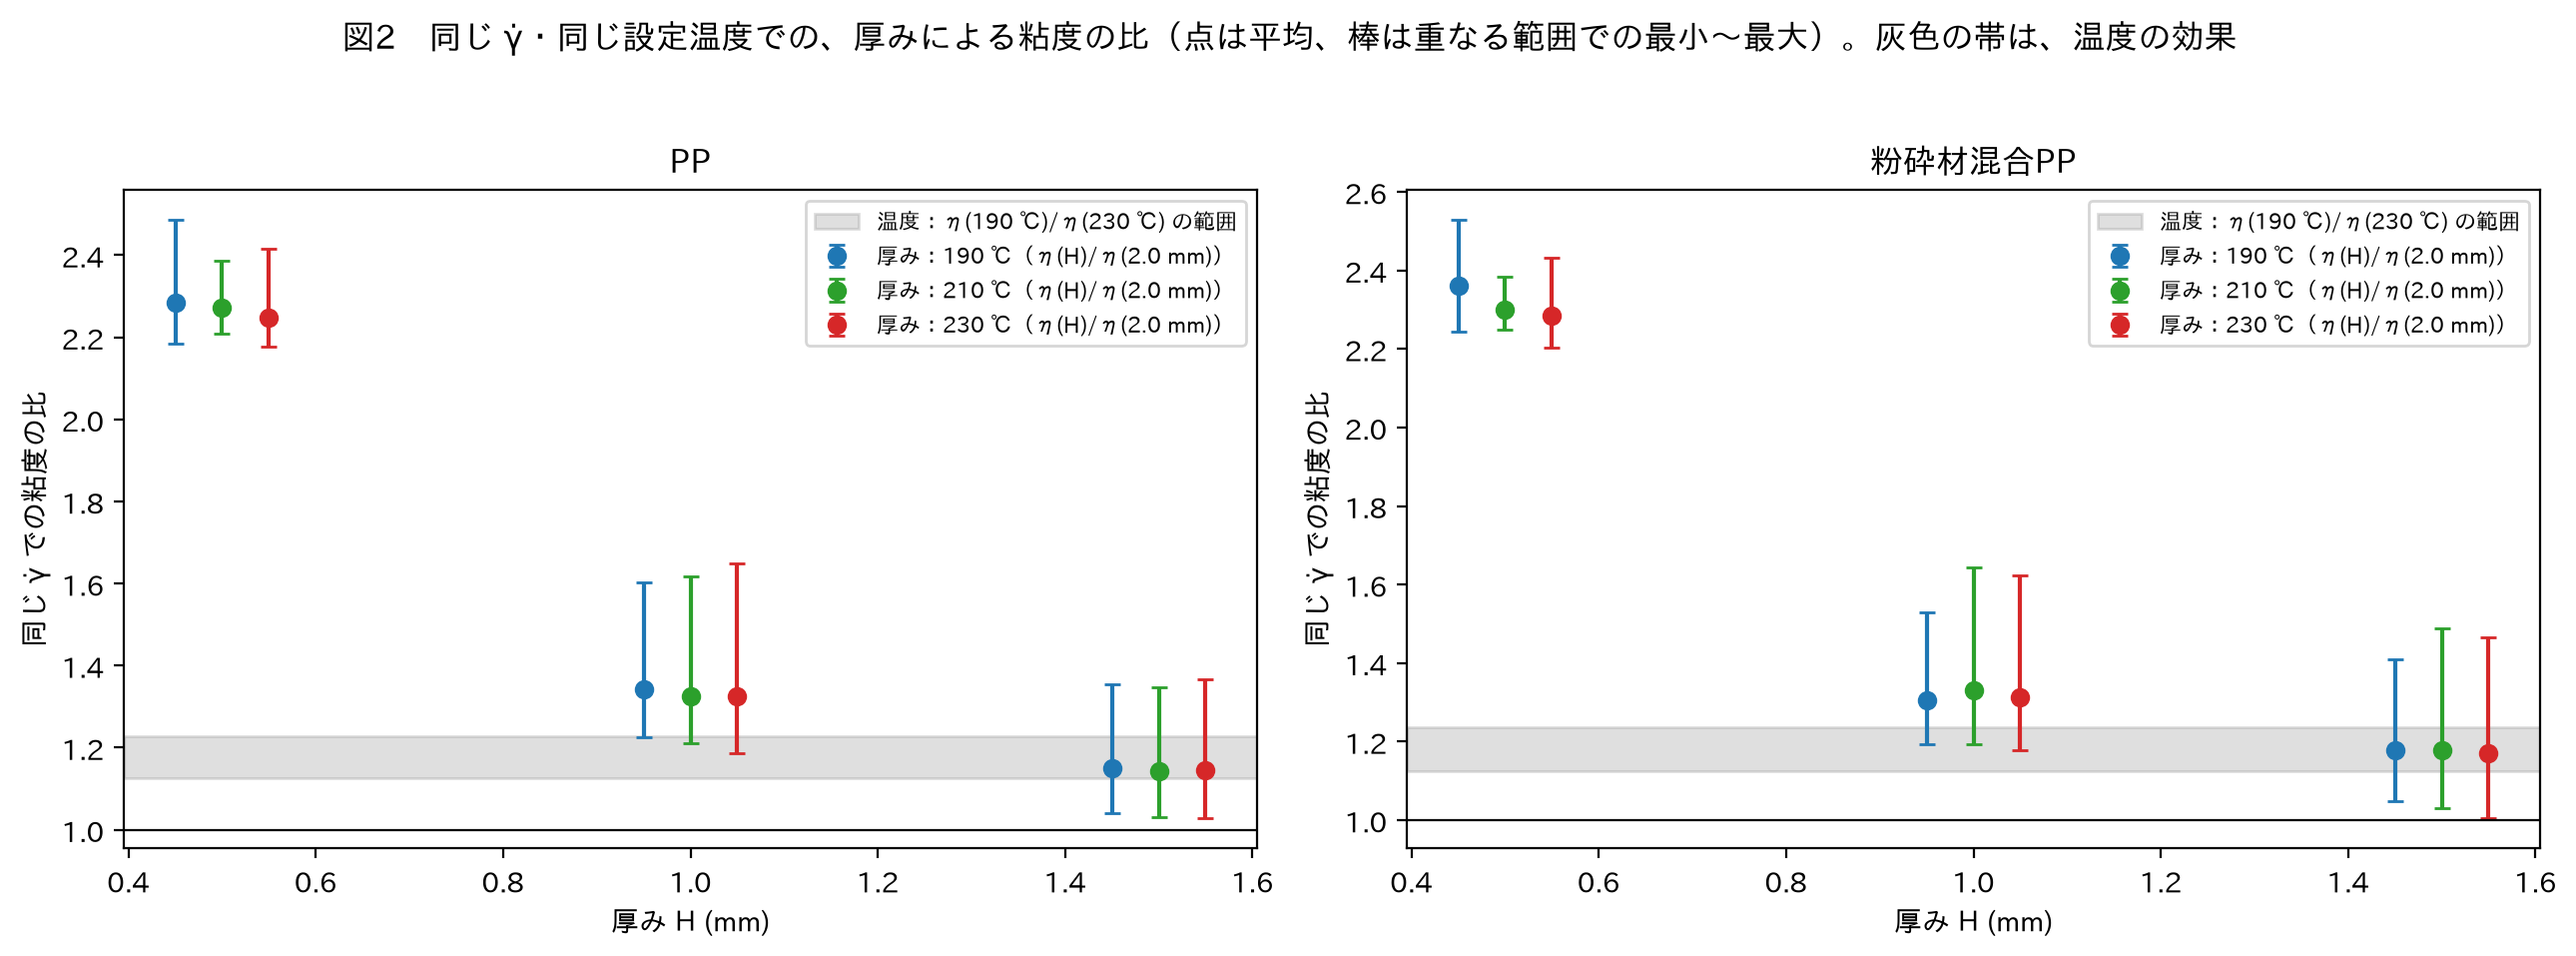
\includegraphics[width=0.95\linewidth]{fig2_thickness_ratio.png}
\caption{同じ $\gd$・同じ設定温度での、厚みによる粘度の比 $\eta(H)/\eta(2.0\,\mathrm{mm})$。灰色の帯は、温度の効果（190 ℃ と 230 ℃ の比）}
\end{figure}
\begin{points}
\pt{何を示す図か}厚みの効果の大きさを、温度の効果と比べる図です。
\pt{軸と記号}横軸は厚み、縦軸は、同じ $\gd$ での粘度の比（基準は 2.0 mm）。点は、$\gd$ が重なる範囲での平均、棒は最小〜最大。色は設定温度。灰色の帯は、同じ厚み・同じ $\gd$ での $\eta(190\,℃)/\eta(230\,℃)$ の範囲。
\pt{見るポイント}点が 1 の線から離れているほど、厚みの効果が大きい。灰色の帯より上なら、温度の効果より大きい。
\pt{今回の結果}厚みによる粘度の比（同じ $\gd$・同じ設定温度）は、0.5 mm で 2.25〜2.36 倍と大きく、厚くなるほど 1 に近づきます。灰色の帯（温度の効果。190 ℃ と 230 ℃ の比 1.12〜1.24 倍）より、厚みの効果のほうが大きいことが分かります。見かけの粘度を予測するには、温度より厚みのほうが効きます。
\end{points}

% ---------------------------------------------------------------------
\subsection{図3：モデルごとの RMSE（\file{fig3\_rmse\_by\_model.png}）}
\begin{figure}[H]
\centering
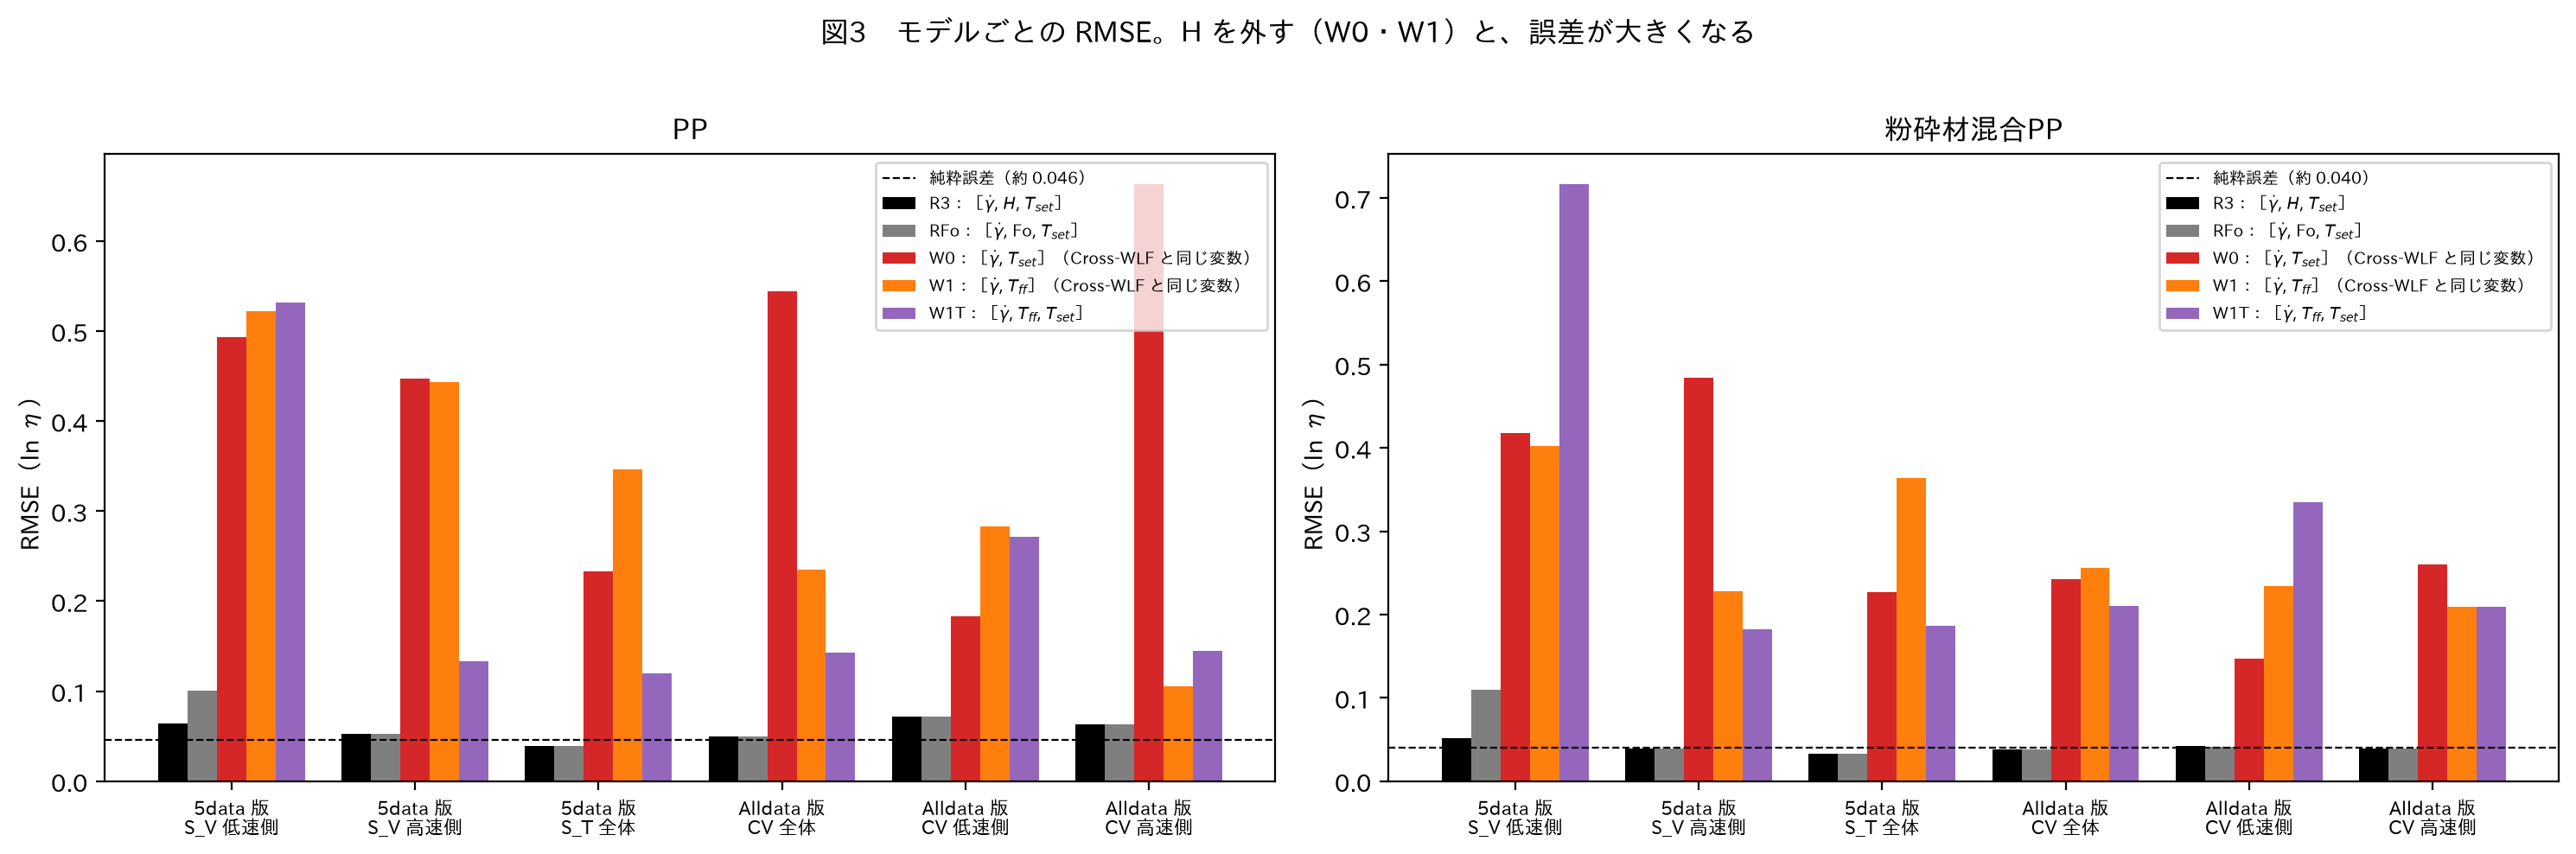
\includegraphics[width=\linewidth]{fig3_rmse_by_model.png}
\caption{モデルごとの RMSE（左 PP、右 粉砕材混合 PP）。破線は純粋誤差}
\end{figure}
\begin{points}
\pt{何を示す図か}$H$ を入れたモデル・外したモデルの誤差を比べる図です。
\pt{軸と記号}横軸は、版・分け方・範囲。棒の色がモデル（黒 R3、灰 RFo、赤 W0、橙 W1、紫 W1T）。破線は純粋誤差。
\pt{見るポイント}(1) R3 が、破線より明らかに下にないか（下ならリークの疑い）。(2) $H$ を外したモデル（W0・W1）が、R3 よりどれだけ悪いか。
\pt{今回の結果}H を入れた R3（黒）と、H を Fo に替えた RFo（灰）は、どこでも純粋誤差（破線）に近い誤差です。H を外した W0（赤）・W1（橙）は、誤差が大きく、S\_T で PP 0.233・0.346（R3 は 0.039）、Alldata 版の CV で PP 0.544・0.235（R3 は 0.049）。2 つの温度を入れた W1T（紫）も、R3 には届きません。
\end{points}

% ---------------------------------------------------------------------
\subsection{図4：厚みごとの残差の平均（\file{fig4\_bias\_by\_thickness.png}）}
\begin{figure}[H]
\centering
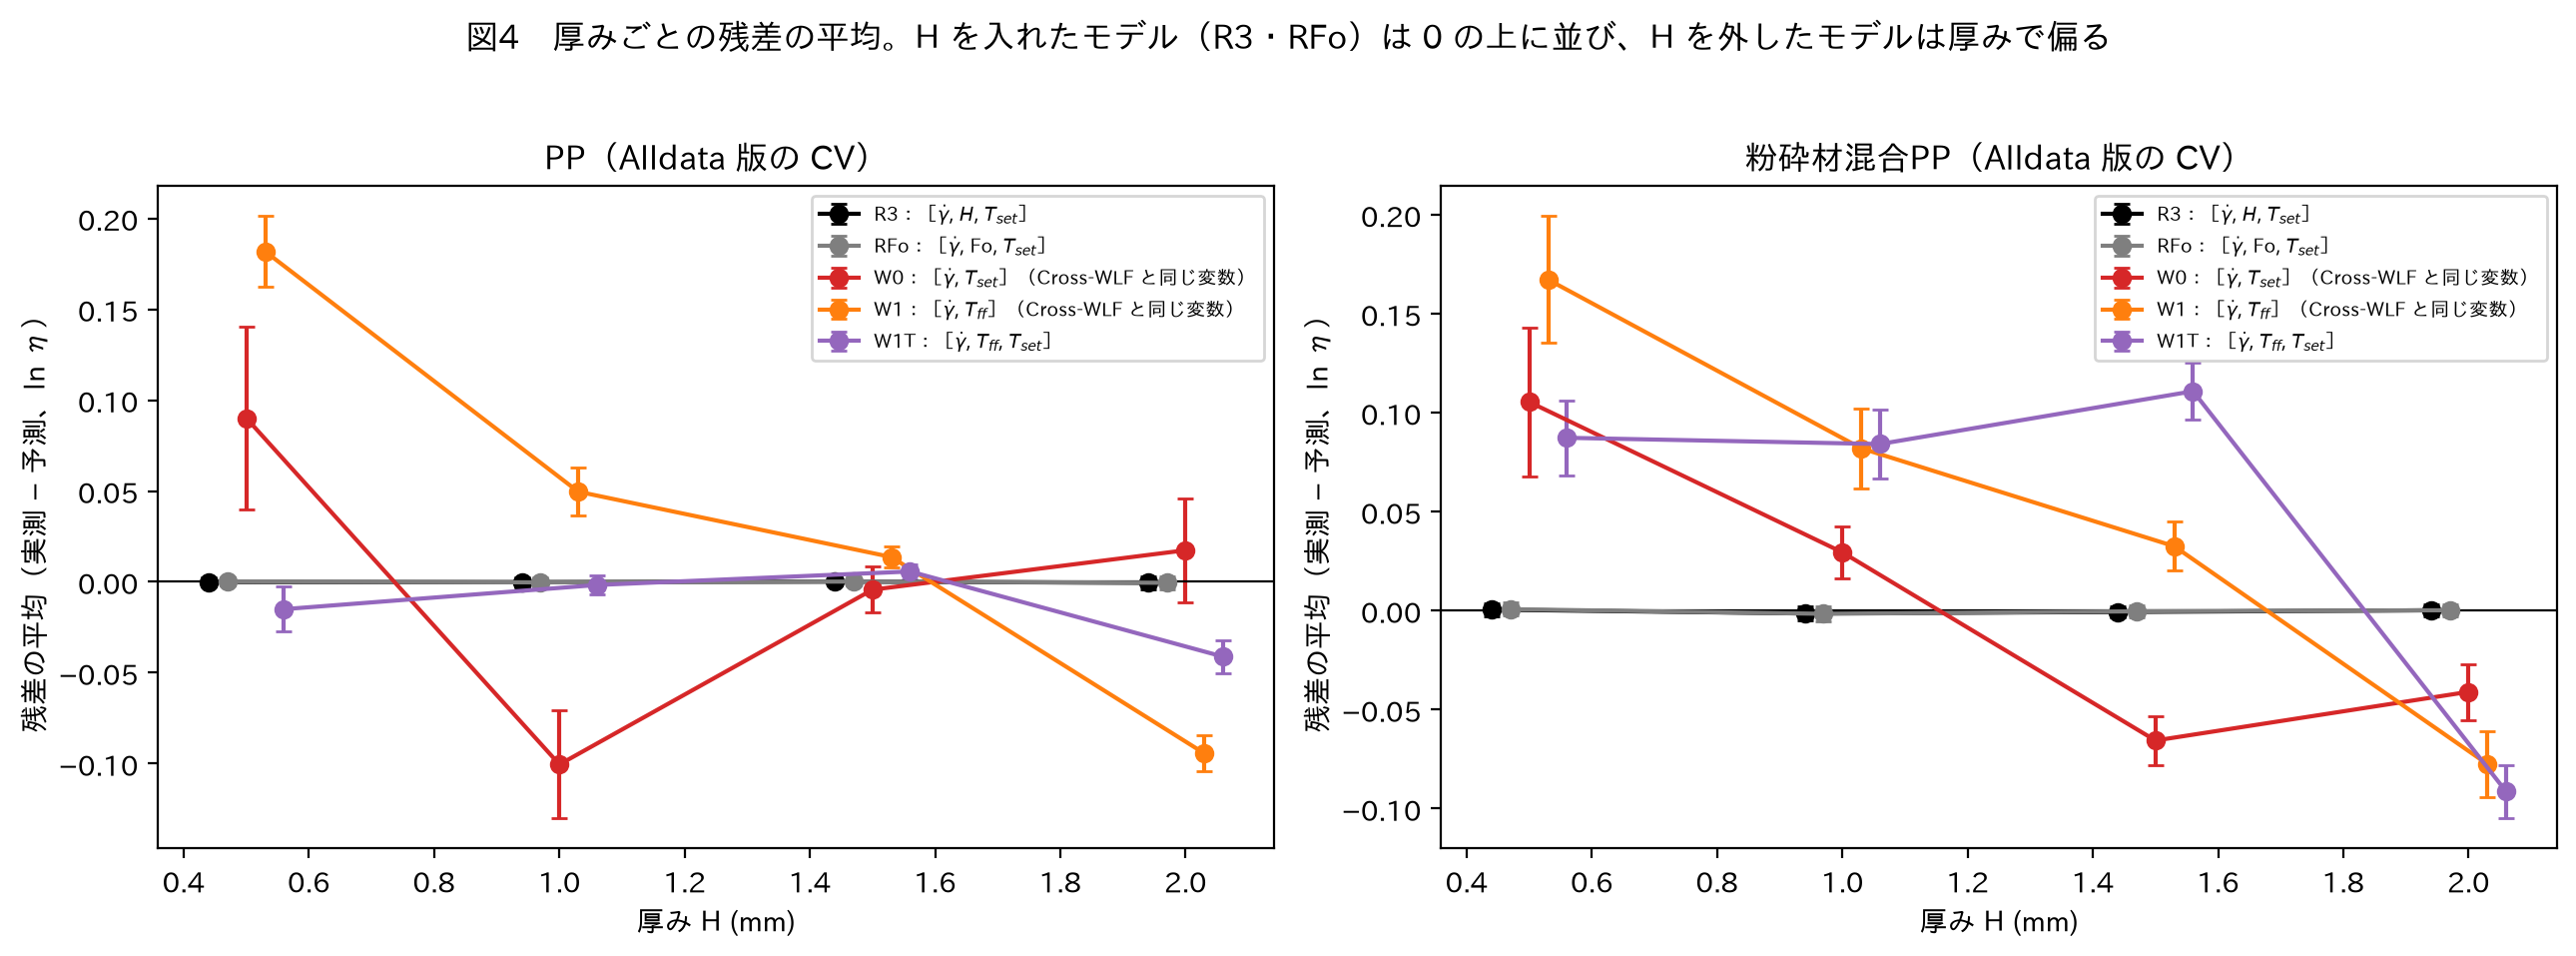
\includegraphics[width=0.95\linewidth]{fig4_bias_by_thickness.png}
\caption{Alldata 版の CV での、厚みごとの残差の平均（実測 $-$ 予測、$\ln\eta$）。棒は標準誤差}
\end{figure}
\begin{points}
\pt{何を示す図か}モデルの誤差が、厚みによって偏っているかを見る図です。
\pt{軸と記号}横軸は厚み、縦軸は残差の平均。色はモデル。
\pt{見るポイント}0 の線の上に並べば、偏りがない。
\pt{今回の結果}R3・RFo は、どの厚みでも残差の平均がほぼ 0 で、厚みの中のばらつき（残差の標準偏差）も 0.03〜0.07 と、純粋誤差と同じくらいです。W0・W1 は、残差の平均が 0 から $\pm$0.1〜0.2 ずれ（W0 の PP：0.5 mm 0.090、1.0 mm $-0.100$、1.5 mm $-0.004$、2.0 mm 0.017）、厚みの中のばらつきが 0.15〜0.80 と、R3 の数倍〜20 倍です。H がないと、GPR は $\gd$ のわずかな違いで条件を見分けて、厚みの違いを無理に当てはめるので、抜いた条件の予測が、上にも下にも大きく外れます（平均すると打ち消し合い、平均だけでは小さく見えます）。5data 版の S\_V（外挿）では、W0 の残差の平均は、どの厚みでも $-$0.25〜$-$0.55 と、一方に偏ります（\file{bias\_by\_thickness.csv}）。
\end{points}

% ---------------------------------------------------------------------
\subsection{高解像度のグラフ（報告書・発表資料用）}
\begin{points}
\pt{ファイル}\file{results/step3e/highres/hr_<材料>_<モデル>_<版>_by-thickness_<厚み>mm.png} と \file{..._by-temperature_<温度>C.png}。既定は、R3・W0・W1 の Alldata 版。Git には入れません。
\pt{見どころ}$H$ を外した W0・W1 は、入力に厚みがないので、設定温度ごとのレイアウトで、4 つの厚みの曲線が 1 本に重なります。実測の点は厚みごとに離れているので、曲線から外れる様子が見えます。
\pt{変え方}ノート7章のセルの先頭の設定エリアで、描くモデル・版などを変えられます（そのセルだけを実行し直せます）。
\end{points}

% =====================================================================
\section{表の見方}

\begin{table}[H]
\caption{算出式に入っている量での線形回帰（ショットごと。5data で学習 $\to$ 3data で検証。\file{formula\_check.csv}）。比：検証の RMSE ／ 純粋誤差（PP 0.041、粉砕材混合 PP 0.039）。リークなら、比がほぼ 0}\label{tab:form}
\begin{tabularx}{\linewidth}{@{}l>{\raggedright\arraybackslash}Xrrr@{}}
\toprule
材料 & 入力 & $\ln H$ の係数 & 検証の RMSE & 比 \\
\midrule
PP & $\ln\gd$, $\ln H$ & $-0.24$ & 0.4720 & 11.54 \\
 & $\ln\gd$, $\ln H$, $\Tset$ & $-0.24$ & 0.4667 & 11.41 \\
 & $\ln\Delta t$, $\ln H$ & 0.99 & 0.4720 & 11.54 \\
 & $\ln\gd$, $\ln H$, $\ln\Delta P$（算出式そのもの） & 1.00 & 0.0001 & 0.00 \\
 & $\ln\gd$, $\ln\Delta P$ & --- & 0.3375 & 8.25 \\
粉砕材混合 PP & $\ln\gd$, $\ln H$ & $-0.24$ & 0.4317 & 10.99 \\
 & $\ln\gd$, $\ln H$, $\Tset$ & $-0.24$ & 0.4252 & 10.83 \\
 & $\ln\Delta t$, $\ln H$ & 0.97 & 0.4317 & 10.99 \\
 & $\ln\gd$, $\ln H$, $\ln\Delta P$（算出式そのもの） & 1.00 & 0.0001 & 0.00 \\
 & $\ln\gd$, $\ln\Delta P$ & --- & 0.3261 & 8.30 \\
\bottomrule
\end{tabularx}
\end{table}

\begin{table}[H]
\caption{同じ $\gd$・同じ設定温度での、厚みによる粘度の比（\file{thickness\_ratio.csv}）。平均（最小〜最大）}\label{tab:ratio}
\begin{tabularx}{\linewidth}{@{}l>{\raggedright\arraybackslash}p{8\zw}XXX@{}}
\toprule
材料 & 比べた厚み & 190 ℃ & 210 ℃ & 230 ℃ \\
\midrule
PP & 0.5 mm / 2.0 mm & 2.28（2.18〜2.49） & 2.27（2.21〜2.39） & 2.25（2.18〜2.42） \\
 & 1.0 mm / 2.0 mm & 1.34（1.23〜1.60） & 1.33（1.21〜1.62） & 1.33（1.19〜1.65） \\
 & 1.5 mm / 2.0 mm & 1.15（1.04〜1.35） & 1.14（1.03〜1.35） & 1.15（1.03〜1.37） \\
 & 190 ℃ / 230 ℃（参考：温度の効果） & \multicolumn{3}{l}{1.12〜1.23（厚みごとの平均の範囲）} \\
粉砕材混合 PP & 0.5 mm / 2.0 mm & 2.36（2.24〜2.53） & 2.30（2.25〜2.38） & 2.29（2.20〜2.43） \\
 & 1.0 mm / 2.0 mm & 1.31（1.19〜1.53） & 1.33（1.19〜1.64） & 1.31（1.18〜1.62） \\
 & 1.5 mm / 2.0 mm & 1.18（1.05〜1.41） & 1.18（1.03〜1.49） & 1.17（1.00〜1.47） \\
 & 190 ℃ / 230 ℃（参考：温度の効果） & \multicolumn{3}{l}{1.12〜1.24（厚みごとの平均の範囲）} \\
\bottomrule
\end{tabularx}
\end{table}

\begin{table}[H]
\caption{モデルごとの RMSE（括弧は被覆率。\file{metrics.csv}）。最後の行は、学習データの純粋誤差}\label{tab:met}
\begin{tabularx}{\linewidth}{@{}l>{\raggedright\arraybackslash}p{4\zw}XXXX@{}}
\toprule
材料 & モデル & 5data 版 S\_V 低速側 & 5data 版 S\_V 高速側 & 5data 版 S\_T & Alldata 版 CV \\
\midrule
PP & R3 & 0.064（1.00） & 0.053（0.88） & 0.039（0.93） & 0.049（0.94） \\
 & RFo & 0.100（1.00） & 0.053（0.86） & 0.039（0.94） & 0.049（0.93） \\
 & W0 & 0.493（1.00） & 0.447（0.91） & 0.233（0.90） & 0.544（0.95） \\
 & W1 & 0.522（0.85） & 0.444（0.85） & 0.346（0.83） & 0.235（0.91） \\
 & W1T & 0.532（0.67） & 0.134（0.56） & 0.120（1.00） & 0.143（0.89） \\
 & 純粋誤差 & 0.041 & 0.041 & 0.040 & 0.051 \\
粉砕材混合 PP & R3 & 0.051（1.00） & 0.039（0.96） & 0.033（0.97） & 0.038（0.96） \\
 & RFo & 0.110（1.00） & 0.039（0.96） & 0.033（0.97） & 0.038（0.96） \\
 & W0 & 0.418（1.00） & 0.484（0.90） & 0.227（0.88） & 0.242（0.92） \\
 & W1 & 0.402（0.91） & 0.228（0.88） & 0.364（0.76） & 0.256（0.92） \\
 & W1T & 0.717（0.36） & 0.182（0.62） & 0.186（1.00） & 0.211（0.95） \\
 & 純粋誤差 & 0.039 & 0.039 & 0.041 & 0.040 \\
\bottomrule
\end{tabularx}
\end{table}

\begin{table}[H]
\caption{厚みごとの残差の平均（Alldata 版の CV。\file{bias\_by\_thickness.csv}）}\label{tab:bias}
\begin{tabularx}{\linewidth}{@{}l>{\raggedright\arraybackslash}p{4\zw}rrrr@{}}
\toprule
材料 & モデル & 0.5 mm & 1.0 mm & 1.5 mm & 2.0 mm \\
\midrule
PP & R3 & 0.000 & 0.000 & 0.000 & $-0.001$ \\
 & RFo & 0.000 & 0.000 & 0.000 & 0.000 \\
 & W0 & 0.090 & $-0.100$ & $-0.004$ & 0.017 \\
 & W1 & 0.182 & 0.050 & 0.014 & $-0.094$ \\
 & W1T & $-0.015$ & $-0.002$ & 0.006 & $-0.041$ \\
粉砕材混合 PP & R3 & 0.001 & $-0.001$ & $-0.001$ & 0.000 \\
 & RFo & 0.001 & $-0.002$ & 0.000 & 0.000 \\
 & W0 & 0.105 & 0.029 & $-0.066$ & $-0.041$ \\
 & W1 & 0.167 & 0.082 & 0.033 & $-0.077$ \\
 & W1T & 0.087 & 0.084 & 0.111 & $-0.091$ \\
\bottomrule
\end{tabularx}
\end{table}

\begin{table}[H]
\caption{長さスケールとノイズの標準偏差（5data 版の S\_V の学習。\file{kernels.csv}）。長さスケールが下限 0.01 に張り付いたモデルは、その入力で条件を見分けている}\label{tab:ls}
\begin{tabularx}{\linewidth}{@{}l>{\raggedright\arraybackslash}p{4\zw}Xr@{}}
\toprule
材料 & モデル & 長さスケール & ノイズ \\
\midrule
PP & R3 & $\gd$ 4.30，$H$ 7.40，$\Tset$ 67.88 & 0.0385 \\
 & RFo & $\gd$ 8.68，Fo 15.50，$\Tset$ 100.00 & 0.0383 \\
 & W0 & $\gd$ 0.01，$\Tset$ 2.90 & 0.0410 \\
 & W1 & $\gd$ 0.01，$\Tff$ 2.50 & 0.0411 \\
 & W1T & $\gd$ 0.24，$\Tset$ 1.85，$\Tff$ 1.59 & 0.0410 \\
粉砕材混合 PP & R3 & $\gd$ 4.10，$H$ 6.87，$\Tset$ 64.94 & 0.0374 \\
 & RFo & $\gd$ 8.04，Fo 14.18，$\Tset$ 100.00 & 0.0373 \\
 & W0 & $\gd$ 0.01，$\Tset$ 2.09 & 0.0395 \\
 & W1 & $\gd$ 0.09，$\Tff$ 0.08 & 0.0393 \\
 & W1T & $\gd$ 0.39，$\Tset$ 2.04，$\Tff$ 0.15 & 0.0393 \\
\bottomrule
\end{tabularx}
\end{table}

% =====================================================================
\section{結果のまとめ}

\subsection{結論：$H$ はリークではない。ただし、見かけの粘度は、厚みに大きく依存する}
\begin{enumerate}[itemsep=0.6ex,topsep=0.6ex]
\item \textbf{H はリークではない（式の面）}：$\ln\eta = \ln\Delta P + \ln H - \ln\gd$ ＋ 定数 なので、H と $\gd$ だけでは、$\Delta P$（流れの結果）が分からず、粘度を計算できません。実際に、$\ln\gd$ と $\ln H$ だけの線形回帰の検証 RMSE は PP 0.47、粉砕材混合 PP 0.43 で、純粋誤差（約 0.04）の 11 倍以上です。$\ln H$ の係数も、式の一部としてだけ効くときの ＋1 ではなく、$-0.24$（PP）でした。$\Delta P$（\PI\ $-$ 0.30 MPa）を足すと、RMSE は 0.0001 と、ほぼ 0 になります（これがリーク。手順3a）。
\item \textbf{H はリークではない（予測の面）}：H は、金型の寸法で、予測するときに事前に分かります。同じ条件のショットで同じ値なので、ショットごとのゆれ（ばらつき）の情報も持っていません。実際に、H を入れた R3 の誤差は、純粋誤差とほぼ同じで、それより小さくはなりません（表\ref{tab:met}）。リークなら、純粋誤差より明らかに小さくなります。
\item \textbf{$\gd$ も、H を使って計算している}：$\gd = 6L/(H\,\Delta t)$ なので、「目的変数の算出に使う値は入力にしない」とすると、Cross-WLF の入力である $\gd$ も使えなくなります。$\gd$ と H を入れることは、測った到達時間 $\Delta t$ と H を入れることと、同じ情報です（表\ref{tab:form} の 1 行目と 3 行目が同じ）。
\item \textbf{見かけの粘度は、厚みで大きく違う}：同じ $\gd$・同じ設定温度で、0.5 mm は 2.0 mm の約 2.25〜2.36 倍の粘度です（図1・図2）。温度の効果（190 ℃ と 230 ℃ で 1.12〜1.24 倍）より大きい効果です。理想的なスリット流れなら、この比は 1 です。
\item \textbf{H を外すと、見かけの粘度を予測できない}：Cross-WLF と同じ変数（$\gd$、$\Tset$）の W0 は、R3 の数倍〜十数倍の誤差です（S\_T で PP 0.233、R3 は 0.039）。温度を、流れの中の樹脂温度 $\Tff$ にした W1 も、同じくらい悪く（0.346）、$\Tff$ では、厚みの効果を説明できません。H を外した GPR は、$\gd$ の長さスケールが下限（0.01）に張り付き、$\gd$ のわずかな違いで条件を見分けて、厚みの違いを無理に説明しようとします（表\ref{tab:ls}）。
\item \textbf{Fo（構造 A・B の入力）は、H と同じ情報}：$\ln\mathrm{Fo} = -(\ln\gd + 3\ln H)$ ＋ 定数 なので、Fo を入れた RFo は、R3 とほぼ同じ精度です（CV：PP 0.049、R3 は 0.049）。手順5a・5本の構造 A・B も、Fo を通して H を使っています。
\end{enumerate}

\subsection{なぜ、見かけの粘度は厚みで違うのか（考えられる理由。この手順では確かめていない）}
理想的なスリット流れと違い、射出成形の流れでは、金型の壁で樹脂が冷やされます。
\begin{points}
\pt{固化層}壁に固化層ができると、流れられる隙間 $H_e = H - 2\delta$（$\delta$ は片側の固化層の厚さ）が、実際の厚み $H$ より狭くなります。見かけの値は $H$ で計算するので、見かけの粘度は、隙間の中の真の粘度の約 $(H/H_e)^2$ 倍に出ます（到達時間から求めた流れの速さを使う場合）。たとえば、両壁に 0.1 mm ずつ固化層があると、0.5 mm では約 2.8 倍、2.0 mm では約 1.2 倍で、その比は約 2.3 倍です。図2 の 0.5 mm / 2.0 mm（2.25〜2.36 倍）と同じくらいの大きさで、薄いほど効く傾向も合います。目安として、熱が壁から樹脂に伝わる深さ $\sqrt{\alpha t}$ は、$\alpha \approx 1\times10^{-7}$ m$^2$/s（樹脂の熱拡散率の目安）、$t \approx 0.07$ s（0.5 mm・$\gd$ 3,000 1/s での到達時間 $\Delta t$）で、約 0.08 mm です（同じ $\gd$ で比べると、薄いほど $\Delta t$ が長い）。ただし、これは大きさの見積もりで、固化層の厚さを測ったわけではありません。
\pt{冷却}薄いほど、また流れる時間が長いほど（フーリエ数 Fo が大きいほど）、樹脂の温度が下がり、粘度が上がります。
\pt{確かめ方}どちらも、厚み方向の温度と固化層の計算（熱の解析）が要ります。このデータだけでは、分けられません。流動先端温度 $\Tff$ を入れても厚みの効果を説明できなかった（W1）のは、$\Tff$ が流れの先端の温度で、隙間全体の温度や固化層の厚さを表さないためと考えられます。
\end{points}

\subsection{ノートの「★要確認」の意味}
ノートの判定で ★ が出るのは、「$H$ を外した W0・W1 の誤差が、R3 の 1.5 倍を超える」ものだけです（材料 2 × 分け方 3 × モデル 2 ＝ 12 件）。これは、「Cross-WLF と同じ変数だけでは、見かけの粘度を予測できない」ことを示す、この手順の主な結果で、エラーではありません。リークの判定（R3 の誤差が純粋誤差より明らかに小さくないか）と、Fo と $H$ の同等性の判定は、すべて OK でした。

\subsection{Cross-WLF と同じ変数のモデルを目指すための選択肢}
Cross-WLF は「材料の式」で、厚みの効果（冷却・固化層）は、流動解析の側が受け持ちます。一方、この研究の目的変数は、それらを含んだ「見かけの粘度」です（CLAUDE.md §2）。そのため、\textbf{Cross-WLF と同じ変数だけで、見かけの粘度を表すことはできません}（W0・W1 の結果）。次の 3 つが考えられます。

\begin{table}[H]
\caption{選択肢}\label{tab:opt}
\begin{tabularx}{\linewidth}{@{}>{\raggedright\arraybackslash}p{8\zw}>{\raggedright\arraybackslash}X>{\raggedright\arraybackslash}p{12\zw}@{}}
\toprule
選択肢 & 内容 & 長所・短所 \\
\midrule
(1) $H$（または Fo）を残す（今の方針） & 見かけの粘度を、$\gd$、$H$（Fo）、$\Tset$ で表す。 & 精度が良い（誤差は純粋誤差と同程度）。リークではない。ただし、材料の式ではなく、このスリットの形の、見かけの値のモデル。 \\
(2) 分ける（材料の部分 ＋ 厚み・冷却の補正） & $\ln\eta = m(\gd, T) + c(\mathrm{Fo})$。$m$ は Cross-WLF と同じ変数の部分（構造 A・B のシフトで温度を入れる）、$c$ は、厚み・冷却の補正（固化層の式などの物理の形か、GP の加法の項）。 & 材料の部分 $m$ が、Cross-WLF にあたる（将来の流動解析に入れる部分）。見かけの粘度の精度も保てる見込み。$m$ と $c$ の分け方が、データだけでは一通りに決まらない心配がある（固化層の式などの、物理の前提が要る）。 \\
(3) $H$ を外す & $\gd$ と温度だけ。 & Cross-WLF と同じ変数。ただし、見かけの粘度の誤差が、数倍〜十数倍になる（厚みの効果が、そのまま誤差になる）。 \\
\bottomrule
\end{tabularx}
\end{table}

\textbf{提案}：ユーザーの目標（Cross-WLF と同じ変数の樹脂粘度モデル）には、(2) が合っています。手順5の本実装で、構造 A・B の「$f(u, \ln\mathrm{Fo})$」を、「$f_1(u) + f_2(\ln\mathrm{Fo})$」（材料の部分 ＋ 補正）に分けた形を足し、(1) と比べることを提案します（$u = \ln\gd + \ln a_T$。$f_1$ が、Cross-WLF の形にあたる曲線）。どれにするかは、ユーザーに決めていただきます。
\end{document}
